\ifx\PREAMBLE\undefined
\documentclass[fleqn]{article}
\usepackage{geometry}
\usepackage[format = hang, font = bf]{caption}
\usepackage{subcaption}
% The following is needed in order to make the code compatible
% with both latex/dvips and pdflatex. Added for using UML generated by MetaUML.
\ifx\pdftexversion\undefined
\usepackage[dvips]{graphicx}
\else
\usepackage[pdftex]{graphicx}
\DeclareGraphicsRule{*}{mps}{*}{}
\fi
\usepackage{array}
\newcolumntype{C}[1]{>{\centering\let\newline\\\arraybackslash}b{#1}}
\newcommand{\parcell}[2][l]{\begin{tabular}{@{}#1@{}}#2\end{tabular}}
\usepackage{pdflscape}
\usepackage{multirow}
\usepackage{graphicx}
\usepackage{floatrow}
\floatsetup[table]{capposition=top}
\usepackage{bigstrut}
\usepackage{supertabular}
\usepackage{booktabs}
\usepackage{amsmath}
\usepackage{listings}
\usepackage{multicol}
\usepackage{xcolor}
\usepackage{mathrsfs}%mathcal
\usepackage{amsfonts}%allowing \mathbb{R}
\usepackage{amssymb}
\usepackage{alltt}
\usepackage{xspace}
\usepackage{color}
\usepackage{wrapfig}%text around figure
\usepackage{lipsum}
\usepackage{tikz}
\usetikzlibrary{shapes,positioning}
\usepackage{url}
\def\UrlBreaks{\do\A\do\B\do\C\do\D\do\E\do\F\do\G\do\H\do\I\do\J\do\K\do\L\do\M\do\N\do\O\do\P\do\Q\do\R\do\S\do\T\do\U\do\V\do\W\do\X\do\Y\do\Z\do\[\do\\\do\]\do\^\do\_\do\`\do\a\do\b\do\c\do\d\do\e\do\f\do\g\do\h\do\i\do\j\do\k\do\l\do\m\do\n\do\o\do\p\do\q\do\r\do\s\do\t\do\u\do\v\do\w\do\x\do\y\do\z\do\0\do\1\do\2\do\3\do\4\do\5\do\6\do\7\do\8\do\9\do\.\do\@\do\\\do\/\do\!\do\_\do\|\do\;\do\>\do\]\do\)\do\,\do\?\do\'\do+\do\=\do\#\do\-}
\usepackage{xr}%allow cross-file references
\usepackage[breaklinks = true]{hyperref}
\lstset{
language = C, 
showspaces = false,
breaklines = true, 
tabsize = 2, 
extendedchars = false, 
basicstyle = {\ttfamily \footnotesize}, 
showstringspaces=false,
keywordstyle=\color{blue!70}, 
commentstyle=\color{gray},
rulesepcolor=\color{red!20!green!20!blue!20}, 
numberstyle=\color[RGB]{0,192,192},
stringstyle=\color{red},
escapeinside={ )},
moredelim=[is][\underbar]{(**}{**)},
mathescape
}
\mathchardef\myhyphen="2D
\begin{document}
\fi
\newpage
\section{Processor Design \& Implementation}
\subsection{Y86-64 ISA}
{\tt
\begin{center}
\tablecaption{Y86-64 instructions}
\tablefirsthead{}
\tablehead{\multicolumn{4}{l}{\small continue}\\}
\tabletail{\multicolumn{4}{r}{\small to be continued}\\}
\tablelasttail{}
\begin{supertabular}{l|C{10pt}|C{10pt}|C{10pt}|C{10pt}|C{140pt}|C{20pt}| }\toprule
{\bf Instruction} & \multicolumn{2}{>{\bf}l|}{0} & \multicolumn{2}{>{\bf}l|}{1} & \multicolumn{1}{>{\bf}l|}{2 - 8} & \multicolumn{1}{>{\bf}l|}{9}\\\midrule
halt 					  & 0 & 0\\\midrule
nop  						& 1 & 0\\\midrule
rrmovq rA rB	  & 2 & 0  & rA & rB\\\midrule
irmovq V rB 		& 3 & 0  & F  & rB & \multicolumn{2}{>{\tt}C{160pt}|}{V}\\\midrule
rmmovq rA D(rB) & 4 & 0  & rA & rB & \multicolumn{2}{>{\tt}C{160pt}|}{D}\\\midrule
mrmovq D(rB) rA & 5 & 0  & rA & rB & \multicolumn{2}{>{\tt}C{160pt}|}{D}\\\midrule
OPq rA rB			  & 6 & fn & rA & rB\\\midrule
jXX Dest				& 7 & fn & \multicolumn{3}{>{\tt}C{160pt}|}{Dest}\\\midrule
cmovXX rA rB		& 2 & fn & rA & rB\\\midrule
call Dest		  	& 8 & 0	 & \multicolumn{3}{>{\tt}C{160pt}|}{Dest}\\\midrule
ret 						& 9 & 0\\\midrule
pushq rA 			  & A & 0	 & rA & F\\\midrule
popq rA 				& B & 0  & rA & F\\\bottomrule
\end{supertabular}
\end{center}

\begin{center}
\tablecaption{Function codes of Y86-64 instructions}
\tablefirsthead{}
\tablehead{\multicolumn{12}{l}{\small continue}\\}
\tabletail{\multicolumn{12}{r}{\small to be continued}\\}
\tablelasttail{}
\begin{supertabular}{C{30pt}|C{10pt}|C{10pt}|C{30pt}|C{10pt}|C{10pt}|C{30pt}|C{10pt}|C{10pt}|C{30pt}|C{10pt}|C{10pt}}\toprule
addq & 6 & 0 & subq & 6 & 1 & andq & 6 & 2 & xorq & 6 & 3\\\midrule
jmp & 7 & 0 & jle & 7 & 1 & jl & 7 & 2 & je & 7 & 3\\\cmidrule(lr){1-12}
jne & 7 & 4 & jge & 7 & 5 & jg & 7 & 6\\\midrule
rrmovq & 2 & 0 & cmovle & 2 & 1 & cmovl & 2 & 2 & cmove & 2 & 3\\\cmidrule(lr){1-12}
cmovne & 2 & 4 & cmovge & 2 & 5 & cmovg & 7 & 6\\\bottomrule
\end{supertabular}
\end{center}

\begin{center}
\tablecaption{Registers in Y86-64 ISA}
\tablefirsthead{}
\tablehead{\multicolumn{8}{l}{\small continue}\\}
\tabletail{\multicolumn{8}{r}{\small to be continued}\\}
\tablelasttail{}
\begin{supertabular}{c|c|c|c|c|c|c|c}\toprule
\%rax & \%rcx & \%rdx & \%rbx & \%rsp & \%rbp & \%rsi & \%rdi\\\cmidrule(lr){1-8}
0 & 1 & 2 & 3 & 4 & 5 & 6 & 7\\\midrule
\%r8 & \%r9 & \%r10 & \%r11 & \%r12 & \%r13 & \%r14 & None\\\cmidrule(lr){1-8}
8 & 9 & A & B & C & D & E & F\\\bottomrule
\end{supertabular}
\end{center}
}
\subsection{SEQ implementation of Y86-64}
\begin{figure}
\centering
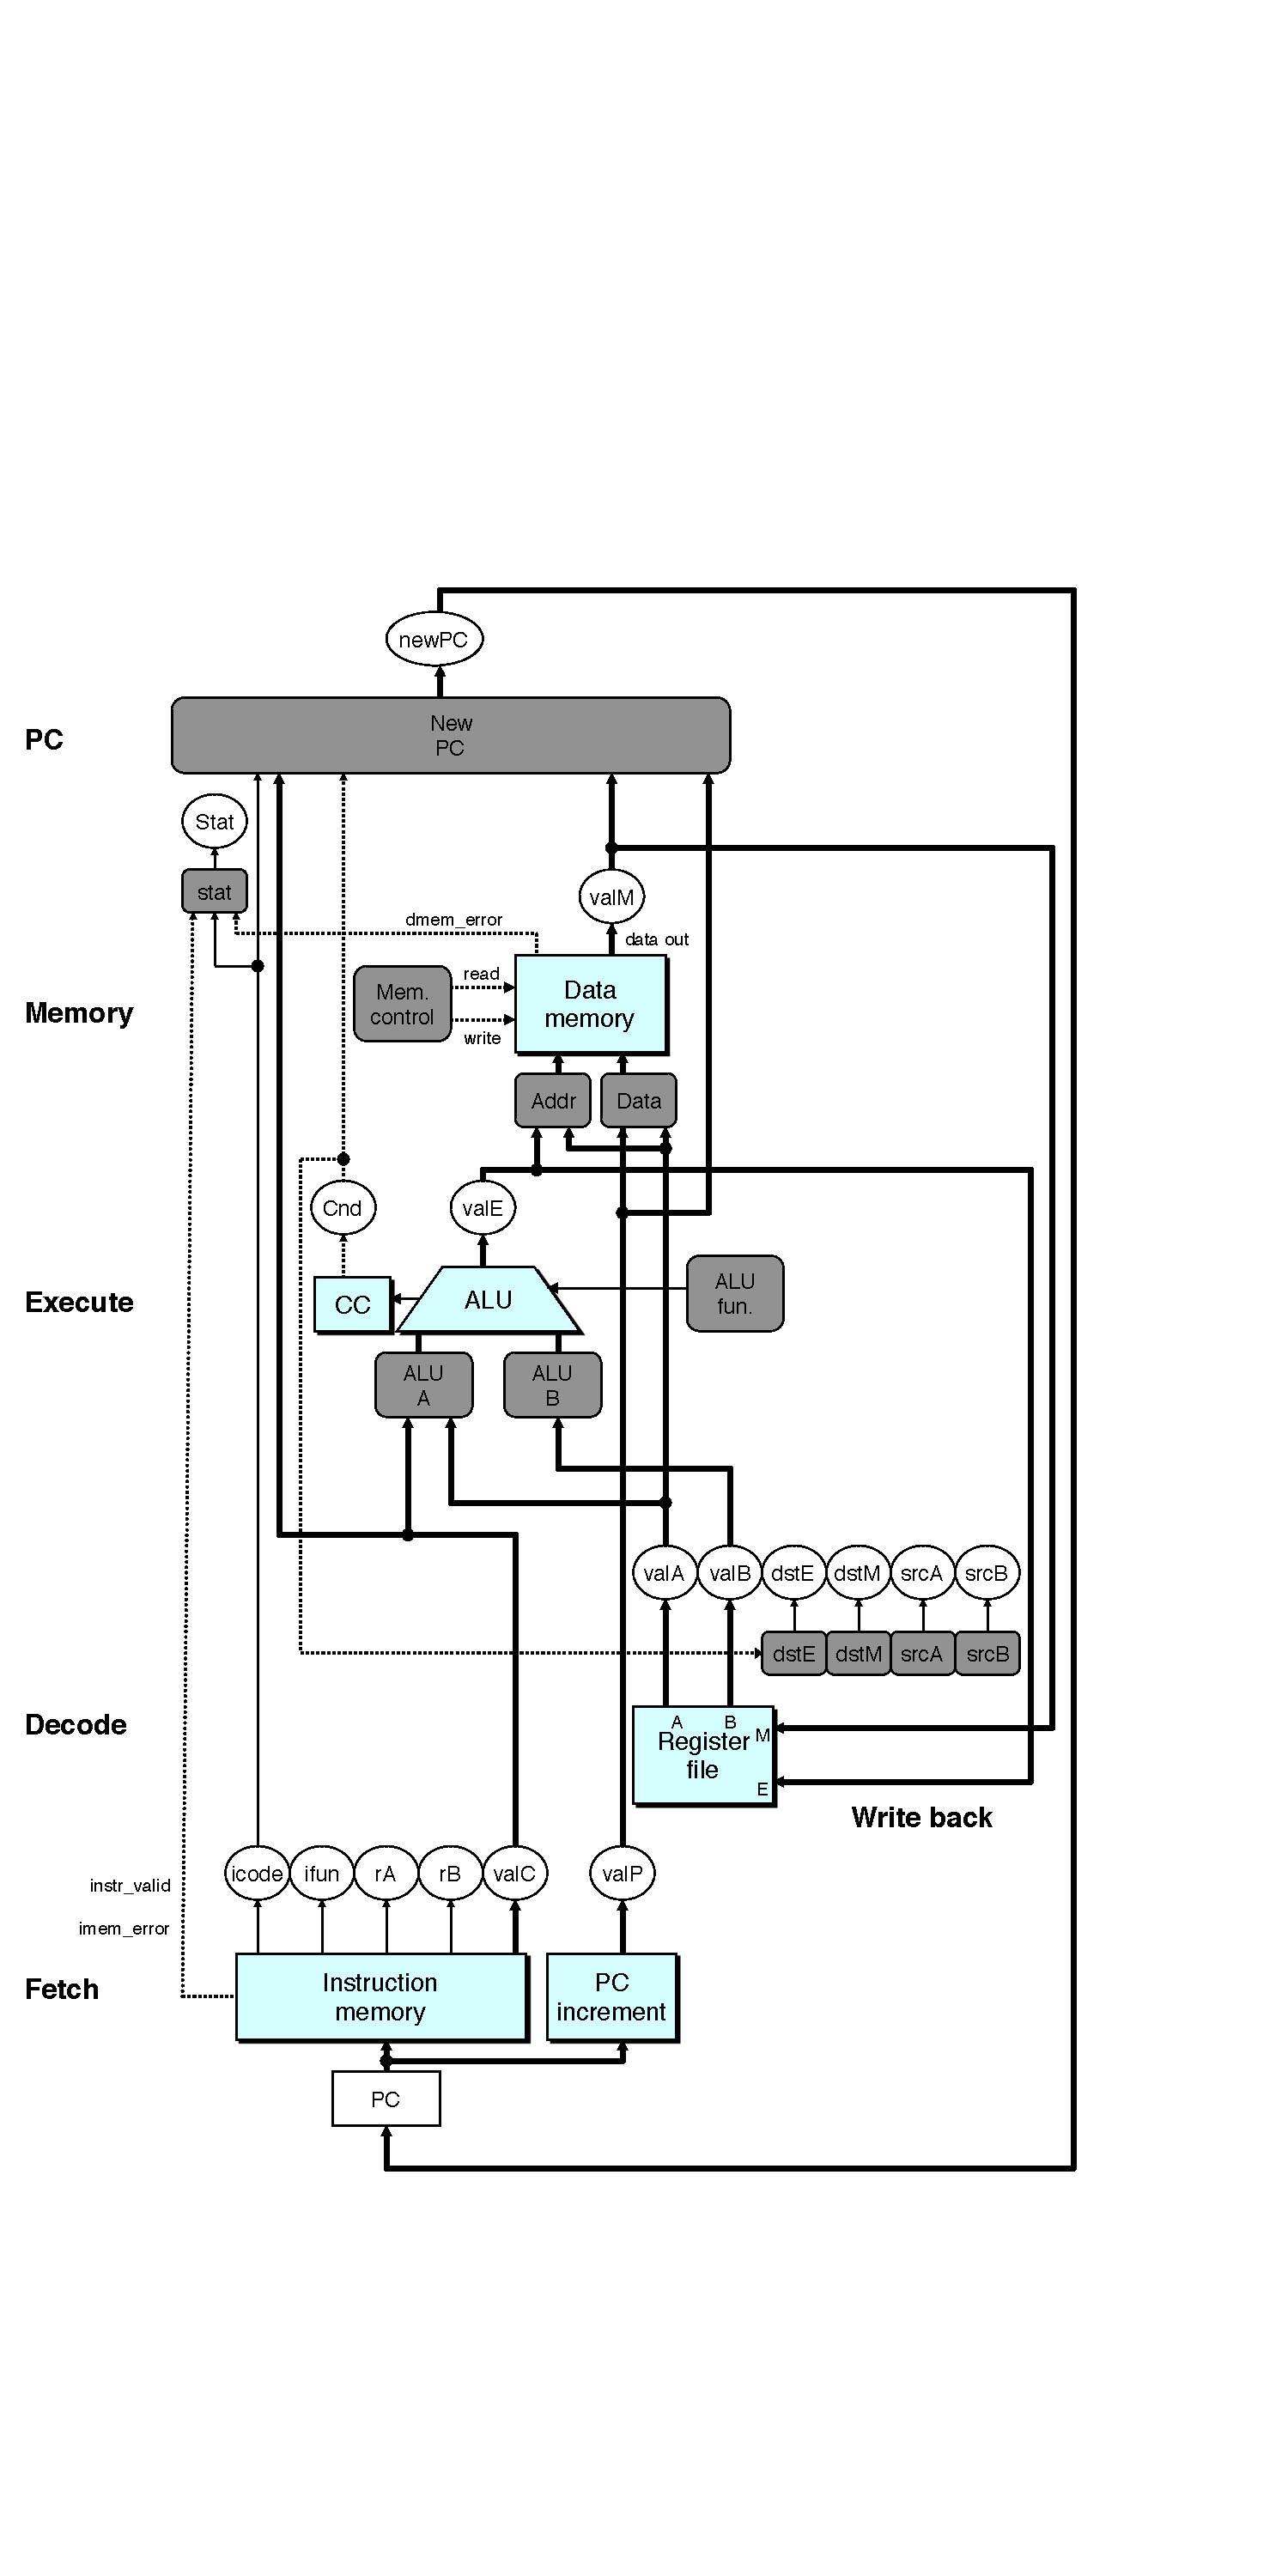
\includegraphics[height=184mm]{seq.pdf}
\caption{Sequential implementation of Y86-64}
\end{figure}
\newgeometry{text={155mm, 220mm}}
{\sffamily
\begin{footnotesize}
\begin{landscape}
\begin{center}
\tablecaption{Sequential implementation of Y86-64}
\tablefirsthead{}
\tablehead{\multicolumn{7}{l}{\small continue}\\}
\tabletail{\multicolumn{7}{r}{\small to be continued}\\}
\tablelasttail{}
\begin{supertabular}{|l|l|l|l|l|l|l|}\toprule
\multicolumn{1}{|>{\bf}c}{Stage} 
& \multicolumn{1}{|>{\bf}c}{Fetch} 
& \multicolumn{1}{|>{\bf}c}{Decode} 
& \multicolumn{1}{|>{\bf}c}{Execute} 
& \multicolumn{1}{|>{\bf}c}{Memory} 
& \multicolumn{1}{|>{\bf}c}{Write Back} 
& \multicolumn{1}{|>{\bf}c|}{PC Update}\\\midrule
OPq rA rB
& \parcell{icode:ifun $\leftarrow$ M$\mathsf{_1}$[PC] \\ rA:rB $\leftarrow$ M$\mathsf{_1}$[PC+1] \\ valP $\leftarrow$ PC+2}
& \parcell{valA $\leftarrow$ R[rA] \\ valB $\leftarrow$ R[rB]}
& \parcell{valE $\leftarrow$ valB OP valA \\ Set CC}
&& R[rB] $\leftarrow$ valE
& PC $\leftarrow$ valP\\\midrule
rrmovq rA rB
& \parcell{icode:ifun $\leftarrow$ M$\mathsf{_1}$[PC] \\ rA:rB $\leftarrow$ M$\mathsf{_1}$[PC+1] \\ valP $\leftarrow$ PC+2}
& valA $\leftarrow$ R[rA]
& valE $\leftarrow$ 0+valA
&& R[rB] $\leftarrow$ valE
& PC $\leftarrow$ valP\\\midrule
irmovq V rB
& \parcell{icode:ifun $\leftarrow$ M$\mathsf{_1}$[PC] \\ rA:rB $\leftarrow$ M$\mathsf{_1}$[PC+1] \\ valC $\leftarrow$ M$\mathsf{_8}$[PC+2] \\ valP $\leftarrow$ PC+10}
&& valE $\leftarrow$ 0+valC
&& R[rB] $\leftarrow$ valE
& PC $\leftarrow$ valP\\\midrule
rmmovq rA D(rB)
& \parcell{icode:ifun $\leftarrow$ M$\mathsf{_1}$[PC] \\ rA:rB $\leftarrow$ M$\mathsf{_1}$[PC+1] \\ valC $\leftarrow$ M$\mathsf{_8}$[PC+2] \\ valP $\leftarrow$ PC+10}
& \parcell{valA $\leftarrow$ R[rA] \\ valB $\leftarrow$ R[rB]}
& valE $\leftarrow$ valB+valC
& M$\mathsf{_8}$[valE] $\leftarrow$ valA
&& PC $\leftarrow$ valP\\\midrule
mrmovq D(rB) rA
& \parcell{icode:ifun $\leftarrow$ M$\mathsf{_1}$[PC] \\ rA:rB $\leftarrow$ M$\mathsf{_1}$[PC+1] \\ valC $\leftarrow$ M$\mathsf{_8}$[PC+2] \\ valP $\leftarrow$ PC+10}
& valB $\leftarrow$ R[rB]
& valE $\leftarrow$ valB+valC
& valM $\leftarrow$ M$\mathsf{_8}$[valE]
& R[rA] $\leftarrow$ valM
& PC $\leftarrow$ valP\\\midrule
pushq rA
& \parcell{icode:ifun $\leftarrow$ M$\mathsf{_1}$[PC] \\ rA:rB $\leftarrow$ M$\mathsf{_1}$[PC+1] \\ valP $\leftarrow$ PC+2}
& \parcell{valA $\leftarrow$ R[rA] \\ valB $\leftarrow$ R[\%rsp]}
& valE $\leftarrow$ valB+(-8)
& M$\mathsf{_8}$[valE] $\leftarrow$ valA
& R[\%rsp] $\leftarrow$ valE
& PC $\leftarrow$ valP\\\midrule
popq rA
& \parcell{icode:ifun $\leftarrow$ M$\mathsf{_1}$[PC] \\ rA:rB $\leftarrow$ M$\mathsf{_1}$[PC+1] \\ valP $\leftarrow$ PC+2}
& \parcell{valA $\leftarrow$ R[\%rsp] \\ valB $\leftarrow$ R[\%rsp]}
& valE $\leftarrow$ valB+8
& valM $\leftarrow$ M$\mathsf{_8}$[valA]
& \parcell{R[\%rsp] $\leftarrow$ valE \\ R[rA] $\leftarrow$ valM}
& PC $\leftarrow$ valP\\\midrule
jXX Dest
& \parcell{icode:ifun $\leftarrow$ M$\mathsf{_1}$[PC] \\ valC $\leftarrow$ M$\mathsf{_8}$[PC+1] \\ valP $\leftarrow$ PC+9}
&& Cnd $\leftarrow$ Cond(CC, ifun)
&&& \parcell{PC $\leftarrow$ Cnd ? \\ valC : valP}\\\midrule
cmoveXX rA rB
& \parcell{icode:ifun $\leftarrow$ M$\mathsf{_1}$[PC] \\ rA:rB $\leftarrow$ M$\mathsf{_1}$[PC+1] \\ valP $\leftarrow$ PC+2}
& valA $\leftarrow$ R[rA]
& \parcell{valE $\leftarrow$ 0+valA \\ Cnd $\leftarrow$ Cond(CC, ifun)}
&& \parcell{if(Cnd)\\R[rB] $\leftarrow$ valE}
& PC $\leftarrow$ valP \\\midrule
call Dest
& \parcell{icode:ifun $\leftarrow$ M$\mathsf{_1}$[PC] \\ valC $\leftarrow$ M$\mathsf{_8}$[PC+1] \\ valP $\leftarrow$ PC+9}
& valB $\leftarrow$ R[\%rsp]
& valE $\leftarrow$ valB+(-8)
& M$\mathsf{_8}$[valE] $\leftarrow$ valP
& R[\%rsp] $\leftarrow$ valE
& PC $\leftarrow$ valC\\\midrule
ret
& \parcell{icode:ifun $\leftarrow$ M$\mathsf{_1}$[PC] \\ valP $\leftarrow$ PC+1}
& \parcell{valA $\leftarrow$ R[\%rsp] \\ valB $\leftarrow$ R[\%rsp]}
& valE $\leftarrow$ valB+8
& valM $\leftarrow$ M$\mathsf{_8}$[valA]
& R[\%rsp] $\leftarrow$ valE
& PC $\leftarrow$ valM\\\bottomrule
\end{supertabular}
\end{center}
\end{landscape}
\end{footnotesize}
}
\restoregeometry
The following design is taken from both the book and the web aside.
\begin{itemize} 
\item Fetch
\begin{lstlisting}
word icode = [
	imem_error : INOP;
	1 : imem_icode;
];
word ifun = [
	imem_error : FNONE;
	1 : imem_ifun;
];
bool instr_valid = icode in {IHALT, INOP, IIRMOVQ, IMRMOVQ, IRMMOVQ, IRRMOVQ, ICALL, IRET, IPUSHQ, IPOPQ, IOPQ, IJXX};
bool need_regids = icode in {IRRMOVQ, IOPQ, IPUSHQ, IPOPQ, IIRMOVQ, IRMMOVQ, IMRMOVQ};
bool need_valC = icode in {IIRMOVQ, IRMMOVQ, IMRMOVQ, ICALL, IJXX};
\end{lstlisting}
valP = PC + 1 + need\_regids + 8 * need\_valC.
\item Decode \& Write Back
\begin{lstlisting}
word srcA = [
	icode in {IRRMOVQ, IRMMOVQ, IOPQ, IPUSHQ} : rA;
	icode in {IPOPQ, IRET} : RRSP;
	1 : RNONE;
];
word srcB = [
	icode in {IOPQ, IRMMOVQ, IMRMOVQ} : rB;
	icode in {IPUSHQ, IPOPQ, ICALL, IRET} : RRSP;
	1 : RNONE;
];
word dstE = [
	icode in {IOPQ, IIRMOVQ} : rB;
	icode == IRRMOVQ && Cnd : rB;
	icode in {ICALL, IRET, IPUSHQ, IPOPQ} : RRSP;
	1 : RNONE;
];
word dstM = [
	icode = {IPOPQ, IMRMOVQ} : rA;
	1 : RNONE;
];
\end{lstlisting}
\item Execute
\begin{lstlisting}
word aluA = [
	icode in {IOPQ, IRRMOVQ} : valA;
	icode in {IIRMOVQ, IRMMOVQ, IMRMOVQ} : valC;
	icode in {IPUSHQ, ICALL} : -8;
	icode in {IPOPQ, IRET} : 8;
];
word aluB = [
	icode in {IOPQ, IRMMOVQ, IMRMOVQ, IPUSHQ, IPOPQ, ICALL, IRET} : valB;
	icode in {IIRMOVQ, IRRMOVQ} : 0;
];
word alufun = [
	icode == IOPQ: ifun;
	1 : ALUADD;
];
bool set_cc = icode in {IOPQ};
\end{lstlisting}
\item Memory
\begin{lstlisting}
bool mem_read = icode in {IMRMOVQ, IPOPQ, IRET};
bool mem_write = icode in {IRMMOVQ, IPUSH, ICALL};
word mem_addr = [
	icode in {IRMMOVQ, IMRMOVQ, IPUSHQ, ICALL} : valE;
	icode in {IPOPQ, IRET} : valA;
];
word mem_data = [
	icode in {IPUSHQ, IRMMOVQ} : valA;
	icode == ICALL : valP;
];
word Stat = [
	imem_error || dmem_error : SADR;
	!instr_valid : SINS;
	icode == IHLT : SHLT;
	1 : SAOK;
];
\end{lstlisting}
\item PC Update
\begin{lstlisting}
word new_pc = [
	icode == ICALL : valC;
	icode == IJXX && Cnd : valC;
	icode == IRET : valM;
	1 : valP;
];
\end{lstlisting}
\end{itemize}
\subsection{Pipeline implementation of Y86-64}
\begin{figure}
\centering
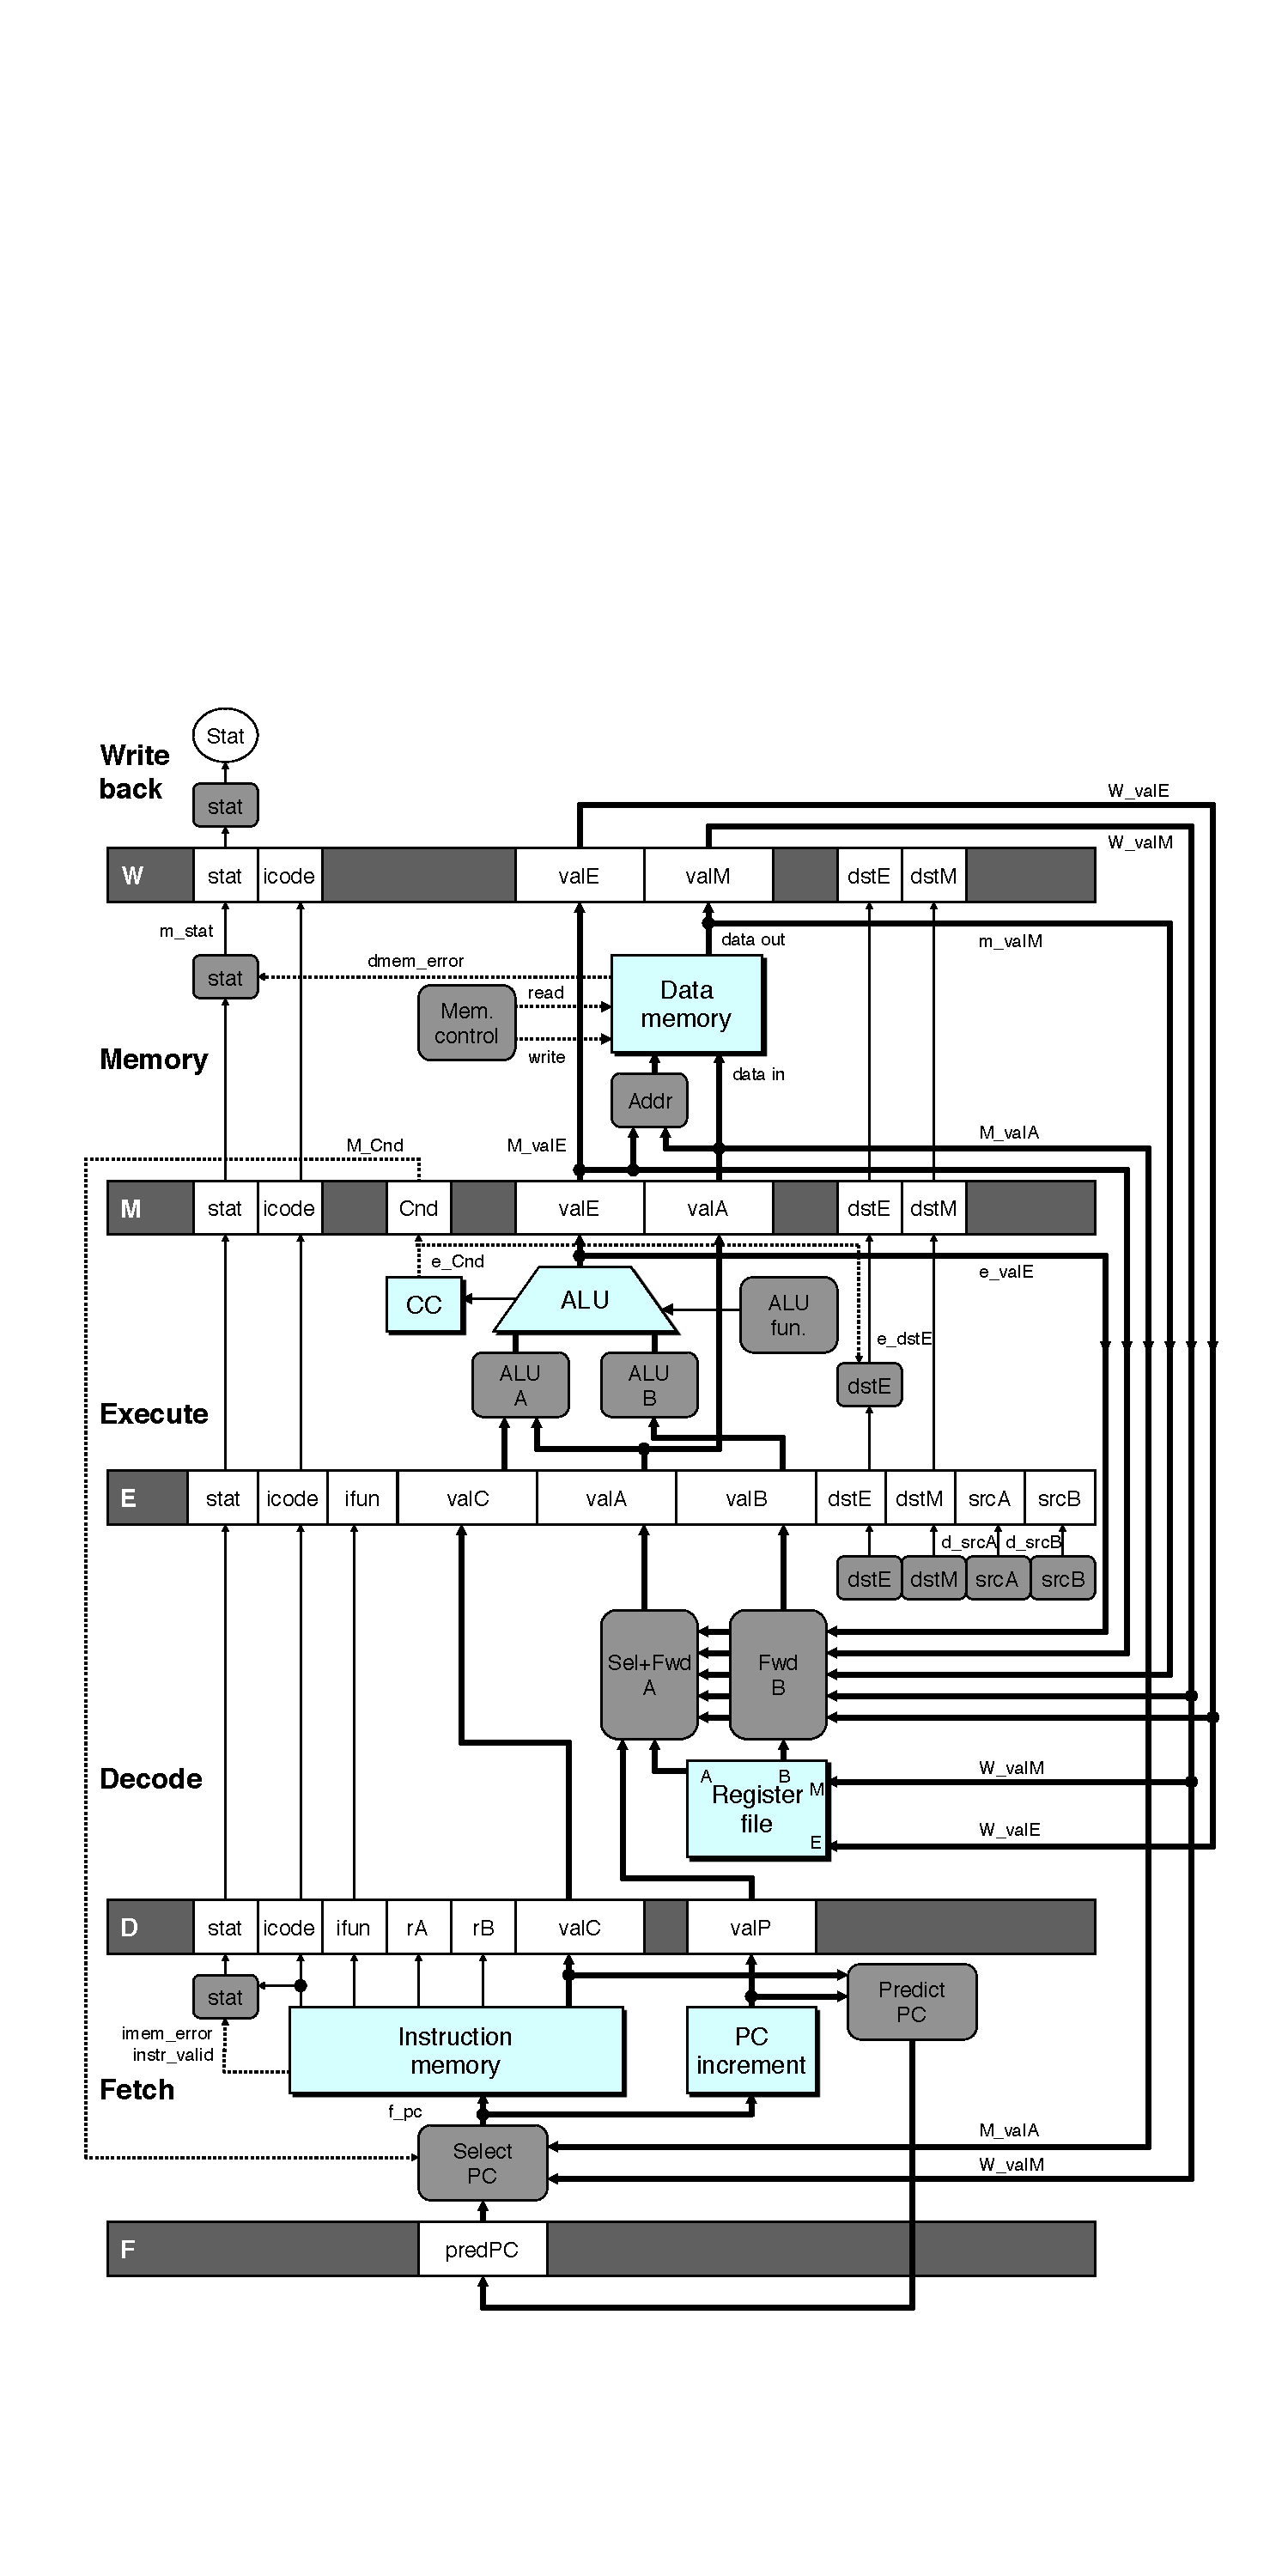
\includegraphics[height=184mm]{pipeline.pdf}
\caption{Pipeline implementation of Y86-64}
\end{figure}
\begin{itemize}
\item Fetch \& PC Selection
\begin{lstlisting}
word f_pc = [
	M_icode == IJXX && !M_Cnd : M_valA; //When jump PC prediction is wrong
	W_icode == IRET : W_valM;
	1 : F_predPC;
];
word f_predPC = [
	f_icode in {IJXX, ICALL} : f_valC; //Strategy for jump PC prediction: always jump
	1 : f_valP;
];
word f_stat = [
	imem_error : SADR; // dmem_error in memory phase
	!instr_valid : SINS;
	f_icode == IHLT : SHLT;
	1 : SAOK;
];

// similar to SEQ
word f_icode = [
	imem_error : INOP;
	1 : imem_icode;
];
word f_ifun = [
	imem_error : FNONE;
	1 : imem_ifun;
];
bool instr_valid = f_icode in {IHALT, INOP, IIRMOVQ, IMRMOVQ, IRMMOVQ, IRRMOVQ, ICALL, IRET, IPUSHQ, IPOPQ, IOPQ, IJXX};
bool need_regids = f_icode in {IRRMOVQ, IOPQ, IPUSHQ, IPOPQ, IIRMOVQ, IRMMOVQ, IMRMOVQ};
bool need_valC = f_icode in {IIRMOVQ, IRMMOVQ, IMRMOVQ, ICALL, IJXX};
\end{lstlisting}
\item Decode \& Write Back

Precedence of forwarding sources:
\begin{itemize}
	\item Forward data affected by the nearest instruction. Thus E $>$ M $>$ W.
	\item For correct behavior of \texttt{popq \%rsp}, M $>$ E.
\end{itemize}
\begin{lstlisting}
word d_valA = [
	D_icode in {ICALL, IJXX} : D_valP;
	d_srcA == e_dstE : e_valE;
	d_srcA == M_dstM : m_valM;
	d_srcA == M_dstE : M_valE;
	d_srcA == W_dstM : W_valM;
	d_srcA == W_dstE : W_valE;
	1 : d_rvalA;
];
word d_valB = [
	d_srcB == e_dstE : e_valE;
	d_srcB == M_dstM : m_valM;
	d_srcB == M_dstE : M_valE;
	d_srcB == W_dstM : W_valM;
	d_srcB == W_dstE : W_valE;
	1 : d_rvalB;
];
word w_dstE = W_dstE;
word w_dstM = W_dstM;
word w_valE = W_valE;
word w_valM = W_valM;
word Stat = [
	W_stat = SBUB : SAOK;
	1 : W_stat;
];
// similar to SEQ
word d_srcA = [
	D_icode in {IOPQ, IRMMOVQ, IRRMOVQ, IPUSHQ} : D_rA;
	D_icode in {IRET, IPOPQ} : RRSP;
	1 : RNONE;
];
word d_srcB = [
	D_icode in {IOPQ, IRMMOVQ, IMRMOVQ} : D_rB;
	D_icode in {IPUSHQ, IPOPQ, ICALL, IRET} : RRSP;
	1 : RNONE;
];
word d_dstE = [
	D_icode in {IOPQ, IIRMOVQ} : rB;
	D_icode in {ICALL, IRET, IPUSHQ, IPOPQ} : RRSP;
	1 : RNONE;
];
word d_dstM = [
	D_icode = {IPOPQ, IMRMOVQ} : D_rA;
	1 : RNONE;
];
\end{lstlisting}
\item Execute
\begin{lstlisting}
bool set_cc = E_icode == IOPQ && !m_stat in {SADR, SHLT, SINS} && !W_stat in {SADR, SHLT, SINS};
word e_valA = E_valA;
word e_dstE = [
	E_icode == IRRMOVQ && !e_Cnd : RNONE;
	1 : E_dstE;
];
// similar to SEQ
word aluA = [
	E_icode in {IOPQ, IRRMOVQ} : E_valA;
	E_icode in {IIRMOVQ, IRMMOVQ, IMRMOVQ} : E_valC;
	E_icode in {IPUSHQ, ICALL} : -8;
	E_icode in {IPOPQ, IRET} : 8;
];
word aluB = [
	E_icode in {IOPQ, IRMMOVQ, IMRMOVQ, IPUSHQ, IPOPQ, ICALL, IRET} : E_valB;
	E_icode in {IIRMOVQ, IRRMOVQ} : 0;
];
word alufun = [
	E_icode == IOPQ: E_ifun;
	1 : ALUADD;
];
\end{lstlisting}
\item Memory
\begin{lstlisting}
word m_stat = [
	dmem_error : SADR;
	1 : M_stat;
];
// similar to SEQ
bool mem_read = M_icode in {IMRMOVQ, IPOPQ, IRET};
bool mem_write = M_icode in {IRMMOVQ, IPUSH, ICALL};
word mem_addr = [
	M_icode in {IRMMOVQ, IMRMOVQ, IPUSHQ, ICALL} : M_valE;
	M_icode in {IPOPQ, IRET} : M_valA;
];
\end{lstlisting}
\end{itemize}
\subsection{Special pipeline control logic}
\begin{table}[ht]
\centering
\caption{Special pipeline control logic}
\begin{tabular} {l|l|c|c|c|c|c}\toprule
& \multicolumn{1}{c|}{\bf Condition} & \textbf{F} & \textbf{D} & \textbf{E} & \textbf{M} & \textbf{W}\\\midrule
ret & \begin{lstlisting}
IRET $\in$ {D_icode, E_icode, M_icode}
\end{lstlisting} 
& stall & bubble & normal & normal & normal\\\midrule
\parcell{load / use\\ hazard} & \begin{lstlisting}
E_icode $\in$ {IMRMOVQ, IPOPQ}
&& E_dstM $\in$ {d_srsA, d_srcB}
\end{lstlisting}
& stall & stall & bubble & normal & normal\\\midrule
\parcell{mispredicted \\ branch} & \begin{lstlisting}
E_icode == IJXX && !e_Cnd
\end{lstlisting} 
& normal & bubble & bubble & normal & normal \\\midrule
exception & \begin{lstlisting}
m_stat $\in$ {SADR, SHLT, SINS} ||
W_stat $\in$ {SADR, SHLT, SINS}
\end{lstlisting} 
& normal & normal & normal & bubble & \parcell[c]{stall\\ (only W)}\\\midrule\midrule
\parcell{ret \& \\ misprediction} & jumps to \texttt{ret} & stall & bubble & bubble& normal & normal\\\midrule
\parcell{ret \& \\ load / use} & set \texttt{\%rsp} followed by \texttt{ret} & stall & stall & bubble & normal & normal \\\bottomrule
\end{tabular}
\end{table}
\begin{lstlisting}
bool F_bubble = 0;
bool F_stall = E_code in {IMRMOVQ, IPOPQ} && E_dstM in {d_srcA, d_srcB} ||
	IRET in {D_icode, E_icode, M_icode};
bool D_stall = E_code in {IMRMOVQ, IPOPQ} && E_dstM in {d_srcA, d_srcB} ||;
bool D_bubble = E_code == IJXX && !e_Cnd ||
	IRET in {D_icode, E_icode, M_icode} && !(E_code in {IMRMOVQ, IPOPQ} && E_dstM in {d_srcA, d_srcB});
bool E_stall = 0;
bool E_bubble = E_code == IJXX && !e_Cnd ||
	E_code in {IMRMOVQ, IPOPQ} && E_dstM in {d_srcA, d_srcB};
bool M_bubble = m_stat in {SADR, SHLT, SINS} ||
	W_stat in {SADR, SHLT, SINS};
bool M_stall = 0;
bool W_bubble = 0;
//Do not stall when m_stat is not OK. Otherwise the instruction in W (which does not cause exception) won't finish.
bool W_stall = W_stat in {SADR, SINS, SHLT};
\end{lstlisting}
\ifx\PREAMBLE\undefined
\end{document}
\fi